

%%%%%%%%%%%%
%
% $Autor: Wings $
% $Datum: 2019-03-05 08:03:15Z $
% $Pfad: Automatisierung/Skript/Produktspezifikation/Powerpoint/AMF.tex $
% $Version: 4250 $
% !TeX spellcheck = en_GB/de_DE
% !TeX encoding = utf8
% !TeX root = filename 
% !TeX TXS-program:bibliography = txs:///biber
%
%%%%%%%%%%%%



\chapter{Training eines Gesichtserkennungsmodells mit Google Colaboratory}
	
%\chapter{TensorFlow Lite mit Portenta H7 verwenden}

In diesem Kapitel werden wir Google Colab verwenden, um ein Objekterkennungsmodell zu trainieren und es dann in das TensorFlow Lite Format zu konvertieren, um es auf den Arduino Portenta H7 hochzuladen und zu validieren. TensorFlow Lite für Mikrocontroller wurde entwickelt, um maschinelle Lernmodelle mit begrenztem Speicher auszuführen. TensorFlow Lite für Mikrocontroller ist in C++ 11 geschrieben und benötigt eine 32-Bit-Plattform.  Das Arduino Portenta H7 Board wird noch nicht unterstützt, um TensorFlow Lite Modelle mit der Arduino IDE \cite{GoogleTensorFlowLite:2021} auszuführen, aber es ist einen Versuch wert.



\subsection{Google Colaboratory}

Google Colaboratory oder Colab ist ein Produkt von Google Research und ist eine kostenlose Jupyter-Notebook-Umgebung, die vollständig in der Cloud läuft. Es ist in der Regel gut für maschinelles Lernen und Datenanalyse geeignet. Das Gute daran ist, dass es keine Einrichtung erfordert und freien Zugang zu Rechenressourcen wie GPU und TPU bietet. \cite{GoogleColab:2021}.

\bigskip


\textbf{Vorteile von Colab} 

\begin{itemize}  
	\item \textbf{Vorinstallierte Bibliotheken:}:
	
	Es bietet vorinstallierte Bibliotheken für maschinelles Lernen, darunter PyTorch, Keras, TensorFlow
	
	\item \textbf{In der Cloud gespeichert:}
	
	Wenn wir ein Jupyter-Notizbuch verwenden, dann wird alles auf einem lokalen Gerät gespeichert. Wenn wir jedoch Google Colab verwenden, können wir es in der Cloud speichern und von jedem Gerät aus darauf zugreifen, indem wir uns einfach beim Google Drive-Konto anmelden.
	
	\item \textbf{Zusammenarbeit:}
	
	Es hilft dabei, mehreren Entwicklern, die an einem Projekt arbeiten, Zugang zu verschaffen, um den Code gemeinsam zu bearbeiten und den fertigen Code mit den Entwicklern zu teilen.
	
	\item \textbf{Kostenlose Nutzung von GPU und TPU:}
	
	Ties ist wahrscheinlich die beste Funktion, denn Google Research lässt uns seine dedizierten GPUs und TPUs für unsere persönlichen Machine-Learning-Projekte nutzen. Daher müssen unsere Computer beim Training des Modells keine komplexen Berechnungen durchführen, da dies in der Cloud geschieht.
	
\end{itemize}


\section{Datenbank}

Die Datenbank für Gesichter ist die gleiche wie im vorherigen Kapitel, nämlich der UTKFace-Datensatz. Wir werden das Modell auf der Grundlage der Bildklassifizierungstechnik trainieren, also werden wir eine andere Klasse verwenden, die in unserem Fall Blumen sind, und die Datenbank dafür kann von Google heruntergeladen werden.

\bigskip

\textbf{Auswahl der Datensätze:} 

Bilder aus dem Blumendatensatz: 100 Bilder von Rosen, die in einem Ordner mit dem Namen \glqq Roses\grqq{} gespeichert sind. Die Abmessungen der Bilder im Datensatz variieren, aber wir wählen Bilder mit Abmessungen im Bereich von $224 \times 224$-Pixel. \ref{DatasetRoses}

\begin{figure}[H]
	\centering
	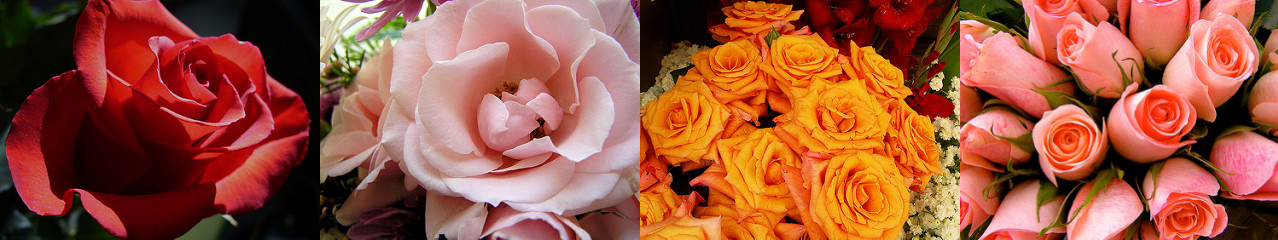
\includegraphics[width=\textwidth]{Arduino/roses}
	\caption{Beispielbilder aus dem Blumendatensatz}
	\label{DatasetRoses}
\end{figure}

\bigskip

Bilder aus dem UTKFace-Datensatz: 120 Bilder, bestehend aus Gesichtern in einem Ordner, der als Faces gespeichert ist. Die Bilder haben eine Größe von $200 \times 200$ Pixel.

\subsection{Verbinden mit Google Drive}

Um ein Notizbuch in Colab zu erstellen und zu speichern, müssen wir es mit unserem Google Drive verbinden. Außerdem müssen wir unseren Bilddatensatz in unser Google Drive hochladen, damit wir von Colab aus darauf zugreifen können. Hierfür verwenden wir die Funktion \PYTHON{drive.mount('/content/gdrive')}. Diese leitet uns zu unserer Google-Anmeldeseite weiter und gibt uns den Autorisierungsschlüssel, den wir benötigen, um unser Google Drive mit Colab zu verbinden. Nach der Eingabe des Schlüssels werden wir mit unserem Google Drive verbunden.


\subsection{Einrichtung des Datensatzes}

Dieser Abschnitt ist ein wichtiger Teil davon, wo wir unsere gezippte Bilddatei und diese .ipynb-Skriptdatei (base\_path) auf unserem Google Drive platziert haben, wie wir unsere gezippte Datei (imagezipped) benannt haben, die in unserem Fall \FILE{images\_RF.zip} ist, und der Name der \SHELL{data\_dir}, der \SHELL{data\_dir='images'} ist, wo wir unsere Bilder vor der Komprimierung kompiliert haben. \ref{GoogleColabDataset}

\begin{figure}[H]
	\centering
	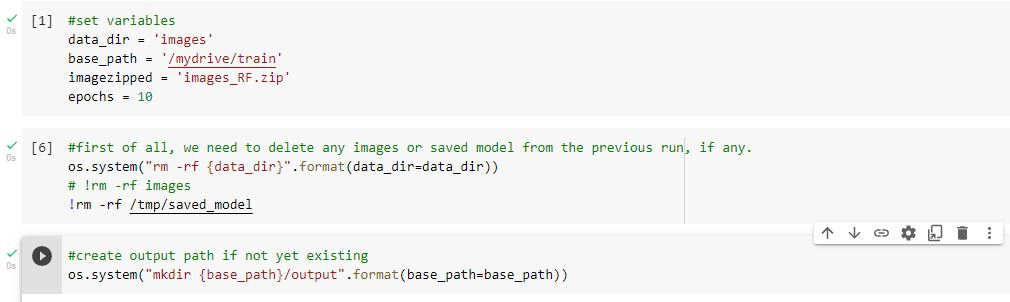
\includegraphics[width=\textwidth]{Arduino/setdataset}
	\caption{Einrichtung des Datensatzes}
	\label{GoogleColabDataset}
\end{figure}

\section{Vorverarbeitung von Daten}

\textbf{Rescaling:}

Im Vorverarbeitungsteil werden wir das Bild zunächst mit der Skalierungsfunktion \PYTHON{rescale=1./255} umskalieren, da unsere Originalbilder aus RGB-Koeffizienten im Bereich von 0-255 bestehen, diese Werte aber für unser Modell zu hoch wären (bei einer typischen Lernrate), so dass wir stattdessen Werte zwischen 0 und 1 anstreben, indem wir mit einem Faktor von 1/255 skalieren. 

\bigskip

\textbf{Datenerweiterung:}

Im Teil der Datenerweiterung werden wir Techniken zur Bildvergrößerung wie das Drehen von Bildern und das horizontale Spiegeln von Bildern verwenden.  In diesem Fall beträgt der Drehbereich der Bilder 40 Grad, wie in Abbildung \ref{GoogleColabAugmentation} dargestellt.

\begin{figure}[H]
	\centering
	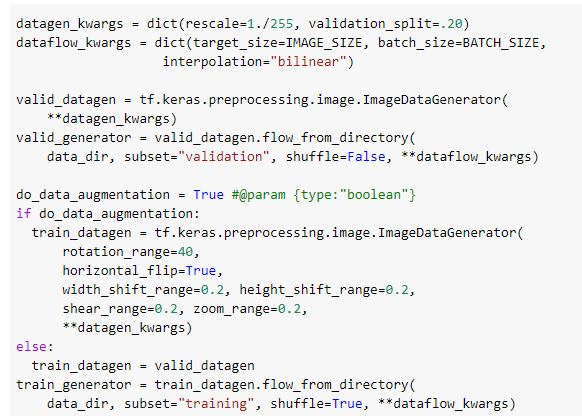
\includegraphics[width=\textwidth]{Arduino/rescaling}
	\caption{Neuskalierung und Datenerweiterung}
	\label{GoogleColabAugmentation}
\end{figure}

\section{Training des Modells}

In diesem Fall haben wir ein vortrainiertes Bildklassifizierungsmodell verwendet, das auf MobileNet V2($224 \times 224$) basiert. Das Eingabebild sollte $224\times 224$ Pixel groß sein. Das Modell wurde mit sequenziellen Keras-Schichten erstellt und die Dropout-Rate beträgt 0,2. Die Stapelgröße beträgt 32 und der in diesem Modell verwendete Optimierer ist Stochastic gradient descent (SGD) mit einer Lernrate von 0,005. Die hier verwendete Verlustfunktion ist die kategoriale Kreuzentropie. Wir haben den Epochenwert auf 10 gesetzt. Epoche ist die Anzahl der Iterationen für die Rückwärtsfortpflanzung, um die Fehler im früheren Teil zu korrigieren, so dass die Genauigkeit erhöht wird. Je größer die Epoche, desto mehr Iterationen und desto länger der Trainingsprozess. \ref{GoogleColabTraining}

\begin{figure}[H]
	\centering
	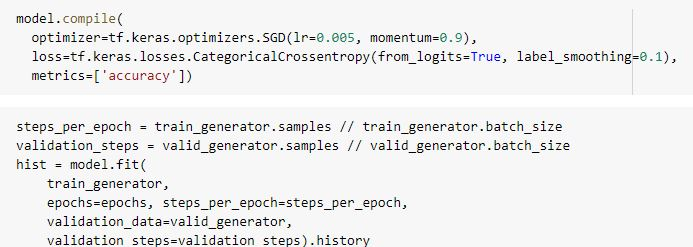
\includegraphics[width=\textwidth]{Arduino/trainingmodel}
	\caption{Training des Modells}
	\label{GoogleColabTraining}
\end{figure}

\section{Prüfung des Modells}

Hier testen wir das Modell an einem Bild aus dem Validierungsdatensatz. Wie in der Abbildung \ref{GoogleColabTesting} zu sehen ist. sagt das Modell die Ausgabe, d. h. das Gesicht im Bild, genau voraus.

\begin{figure}[H]
	\centering
	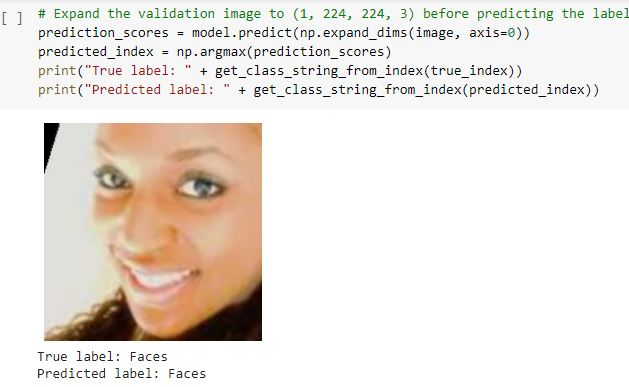
\includegraphics[width=\textwidth]{Arduino/testing}
	\caption{Prüfung des Modells}
	\label{GoogleColabTesting}
\end{figure}

Das trainierte Modell kann dann auf dem Sitzungsspeicher abgelegt werden.

\section{Umwandlung des gespeicherten Modells in das tflite-Format}

Um das gespeicherte Modell in das TFLite-Format zu konvertieren, verwenden wir die folgende Funktion \PYTHON{converter = tf.lite.TFLiteConverter.from\_saved\_model(saved\_model)}

Nach der Konvertierung des Modells in tflite speichern wir die tflite-Datei auf unserem Laufwerk. Der nächste Schritt ist die Konvertierung der tflite-Datei in das C++-Format, damit wir das Programm in die Arduino-IDE hochladen können.

\section{Konvertierung der tflite-Datei in eine Arduino-Header-Datei}

Um das Objekterkennungsmodell in der Arduino-IDE ausführen zu können, müssen wir unser Modell im C++-Format programmieren und außerdem die aus unserem tflite-Modell erstellte Arduino-Header-Datei hinzufügen. Um eine Arduino-Header-Datei zu erstellen, verwenden wir Gitpod, um die tflite-Datei in eine Header-Datei (.h-Datei) zu konvertieren. Dazu müssen wir uns zunächst mit unseren GitHub-Anmeldedaten bei GitPod anmelden. Dann müssen wir einen neuen Arbeitsbereich erstellen. Im Befehlsterminal müssen wir diesen Befehl \PYTHON{xxd -i model.tfite model.h} verwenden.

Dadurch wird eine Header-Datei erzeugt, die wir in unserem C++-Programm benötigen, um sie in die Arduino-IDE hochzuladen. Nachdem wir die Header-Datei heruntergeladen haben, müssen wir den Inhalt der Datei kopieren und mit dem Befehl \PYTHON{const unsigned char model\_tflite[] = } in unser Programm einfügen. Dies stellt die Merkmale unseres Gesichtserkennungsmodells dar. Dann müssen wir die Gesichtserkennungsfunktion in C++-Code implementieren.

\section{Offene Fragen}

\subsection{Arduino Portenta H7-Board nicht kompatibel für Objekterkennung mit Arduino IDE}

Das Problem, das bei der Implementierung des Gesichtserkennungsmodells mit der Arduino IDE auftrat, ist, dass es keine früheren Arbeiten zur Objekterkennung mit dem Arduino Portenta H7-Board gab, da es nicht kompatibler war, so dass keine Daten verfügbar waren, die als Referenz für unser Gesichtserkennungsmodell verwendet werden konnten.\cite{GoogleTensorFlowLite:2021} Auch die Implementierung eines TensorFlowLite Modells in der Arduino IDE ist eine schwierige Aufgabe, da unser Board nicht schnell genug ist und die Zeit zum Kompilieren eines Programms mehr als 20 Minuten beträgt und es keine Bibliotheken zur Implementierung des Objekterkennungsmodells gibt. Es gibt jedoch nur ein einziges online verfügbares Beispiel, das Hello World-Beispiel von Arduino, das auch als Sinuswellenfunktion im Tflite-Format bezeichnet wird und mit der Arduino-IDE ausgeführt werden kann, aber wir können dies nicht als Referenz nehmen, da das Objekterkennungsmodell und das Sinuswellenmodell völlig unterschiedlich sind. 

\subsubsection{Mögliche Lösung}

Die mögliche Lösung könnte die Verwendung von OpenMV IDE anstelle von Arduino IDE sein. OpenMV IDE hat im Vergleich zu Arduino IDE mehr Funktionen, wie z.B. das Hochladen von Datensätzen in Echtzeit durch die Erfassung von Bildern vom Vision Shield. Es hat auch viele weitere Beispielprogramme wie Gesichtsverfolgung, Gesichtsfilter. Daher könnte die Verwendung von OpenMV IDE eine bessere und einfache Lösung für dieses Problem sein. 

\subsection{Einsatz des auf Edge Impulse trainierten Objekterkennungsmodells mit Arduino IDE nicht möglich }

Das Objekterkennungsmodell, das für die Gesichtserkennung in der Edge-Impulse-Plattform trainiert wurde, und die online generierte tflite-Datei konnten nicht auf der Arduino IDE eingesetzt werden. Das Modell funktioniert auf der Plattform einwandfrei, doch bei der Bereitstellung auf dem Arduino Portenta H7-Board unter Verwendung der Arduino IDE traten verschiedene Fehler auf. Nach Rücksprache mit den Edge-Impulse-Plattform Schöpfer haben wir zu wissen, dass sie noch nicht bereit sind, in den Einsatz des Modells von ihrer Plattform mit Arduino IDE generiert.

\subsubsection{Mögliche Lösung}

Das von der Edge Impulse-Plattform generierte Modell ist in der Programmiersprache Python kodiert. Für die Arduino IDE ist die Programmiersprache C++. Daher hat Edge Impulse ab sofort einige Probleme mit der Arduino IDE, da einige Änderungen vorgenommen werden müssen. Die bessere Lösung wäre also die Verwendung der OpenMV IDE, da sie MicroPython unterstützt und das Edge Impulse-Modell eine Python-Datei erzeugt, die wir in die OpenMV IDE hochladen und unser Gesichtserkennungsmodell implementieren können.


\chapter{Quellcode}




\section{Face Detection using Edge Impulse and OpenMV}

\begin{verbatim}
	import sensor, image, time, os, tf
	
	sensor.reset()                         # Reset and initialize the sensor.
	sensor.set_pixformat(sensor.GRAYSCALE)    # Set pixel format to RGB565 (or GRAYSCALE)
	sensor.set_framesize(sensor.QVGA)      # Set frame size to QVGA (320x240)
	sensor.set_windowing((240, 240))       # Set 240x240 window.
	sensor.skip_frames(time=2000)          # Let the camera adjust.
	
	net = "trained.tflite"
	labels = [line.rstrip('\n') for line in open("labels.txt")]
	
	clock = time.clock()
	while(True):
	clock.tick()
	
	img = sensor.snapshot()
	
	# default settings just do one detection... change them to search the image...
	for obj in tf.classify(net, img, min_scale=1.0, scale_mul=0.8, x_overlap=0.5, y_overlap=0.5):
	print("**********\nPredictions at [x=%d,y=%d,w=%d,h=%d]" % obj.rect())
	img.draw_rectangle(obj.rect())
	# This combines the labels and confidence values into a list of tuples
	predictions_list = list(zip(labels, obj.output()))
	
	for i in range(len(predictions_list)):
	print("%s = %f" % (predictions_list[i][0], predictions_list[i][1]))
	
	print(clock.fps(), "fps")
	
\end{verbatim}



